\chapter{無線タグおよびMQTTプロトコルを用いた計測システム}

\section{はじめに}
この章では今回使用するシステムの構成についてまとめた.

\section{無線タグTWELITE}
\subsection{TWELITEの諸元}
無線タグTWELITEの通信は親機としてMONOSTICK,子機としてTWELITE CUEという機器を使用して行われる.各機器の諸元は表\ref{twelite}の通りである.

親機・子機間の通信は2.4GHz IEEE 802.15.4 に準拠して行われ,変調方式はO-QPSK, DSSSである.\cite{TWdatasheet}
親機MONOSTICKは多数の子機からの情報を受信でき,PCにはシリアルポートとして認識される.
そのため,多くのOSで利用可能である.
子機には加速度センサーが搭載されていて,その測定値を送信することができる.
親機を接続したPC・マイコン等はその情報を確認できるほか,子機から送信された電波がどのくらいの強度で届いたかを後述のLQ値という指標を用いて表示する.\cite{TW1}
子機から親機への送信頻度の設定は加速度サンプリング頻度と加速度送信サンプル数を変化させることにより行え,
サンプリング頻度が25Hz,送信サンプル数が16の時の送信頻度は25/16($\fallingdotseq$1.56)Hzである.
本稿では,電波強度が親機と子機との距離に応じて変化することに着目して実験を行う.

\begin{table}[htb]
 \centering
 \caption{TWELITE諸元}
  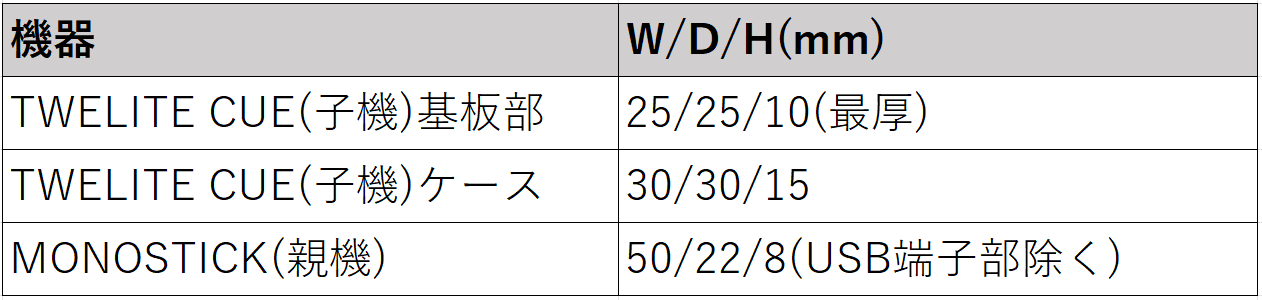
\includegraphics[width = 12cm, bb= 0 0 900 250]{chapter2/TWELITE.png}
   
  \label{twelite}
\end{table}


\subsection{LQ値}
LQ(Link\ Quality)値とはモノワイヤレス社製品における通信品質を表す値で,
LQ値150以上は送信機の近傍にいること,50未満は通信品質が著しく悪いこと(-80dBm)を示す.
以下の式でdBmと変換することができる.\cite{TWLQ}

\begin{equation}
  dBm = (7*LQ-1970)/20
\end{equation}

本研究では,電波強度を評価するための指標としてこのLQ値を用いる.



\section{MQTTプロトコル}
MQTT(MQ\ Telemetry\ Transport)プロトコルは,小型デバイス間でのメッセージ交換用に設計されたTCP/IP(ポート1883)を使用するプロトコルである.
メッセージを確実に送信することを目的としているため,プロトコルヘッダが小さいことが特徴で,即時性,軽量さが長所として挙げられる.\cite{MQTT}
通信環境は,図\ref{mqtt}のように,メッセージを送信する側のパブリッシャと受信する側のサブスクライバに加え,中継者としてのブローカーから構成される.
通信はパブリッシャがブローカーにメッセージを送信し,サブスクライバがブローカーから必要なメッセージを受信するという方式により行われる.
必要なメッセージのみを受信する方法として,TOPICという識別子が用いられている.
パブリッシャはメッセージにTOPICを付加し,サブスクライバは受信するTOPICを設定する.
ブローカーはパブリッシャから受信したデータについて,付加されたTOPICを受信する設定をしているサブスクライバのみにメッセージを送るという仕組みによりサブスクライバが不必要なメッセージまで受信することを防いでいる.
本研究では,MONOSTICKを接続しているマイコン(Raspberry Pi)をパブリッシャ,マイコンとLANを通して接続されたPCをサブスクライバとする.
片方向,かつ集約的な通信を行う本研究において,ブローカーはサブスクライバのPCと兼ねて差し支えないため,
サブスクライバPCにブローカー($\text{Eclipse Mosquitto}^\text{TM}$)を導入して通信を行う.

\begin{figure}[!htb]
  \centering
  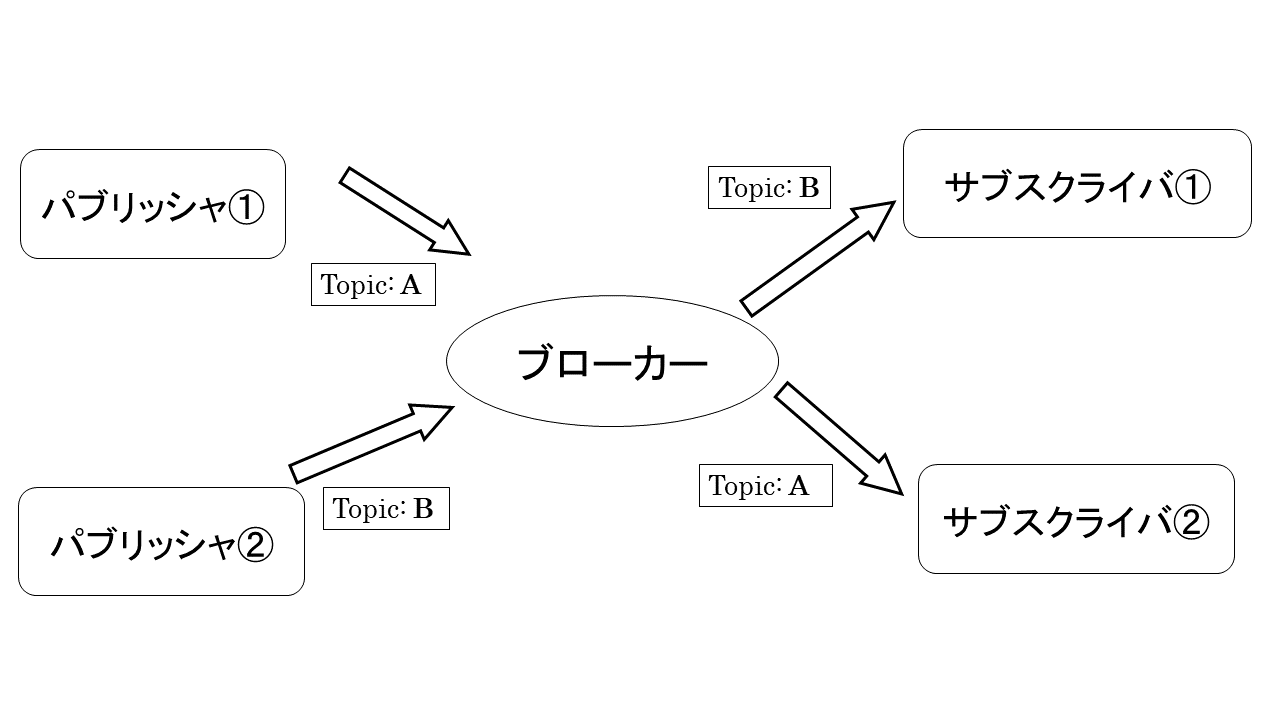
\includegraphics[width = 12cm, bb= 0 0 900 600]{chapter2/MQTT.png}
  \caption{MQTT構成の概要}
  \label{mqtt}
\end{figure}

\clearpage


\section{計測システムの構成}
本研究では,これまでに述べた機器・プロトコルを用いて,プレーパークや保育園において図\ref{system}のようなシステムを構成する.
子供につけたTWELITE無線タグから発信されたデータは,各遊具・遊び場にあるマイコンに接続されたMONOSTICK及びMQTTプロトコルを介して,
子供が”いつ”,”どの遊具・遊び場を使っていたか”がわかるデータとして集積される.
そのうえで,集積されたデータから子供の動きを解析し,個性や交友関係について定量的な分析を行うことを可能にし,より高度な教育につなげることを目指す.



\begin{figure}[!htb]
  \centering
  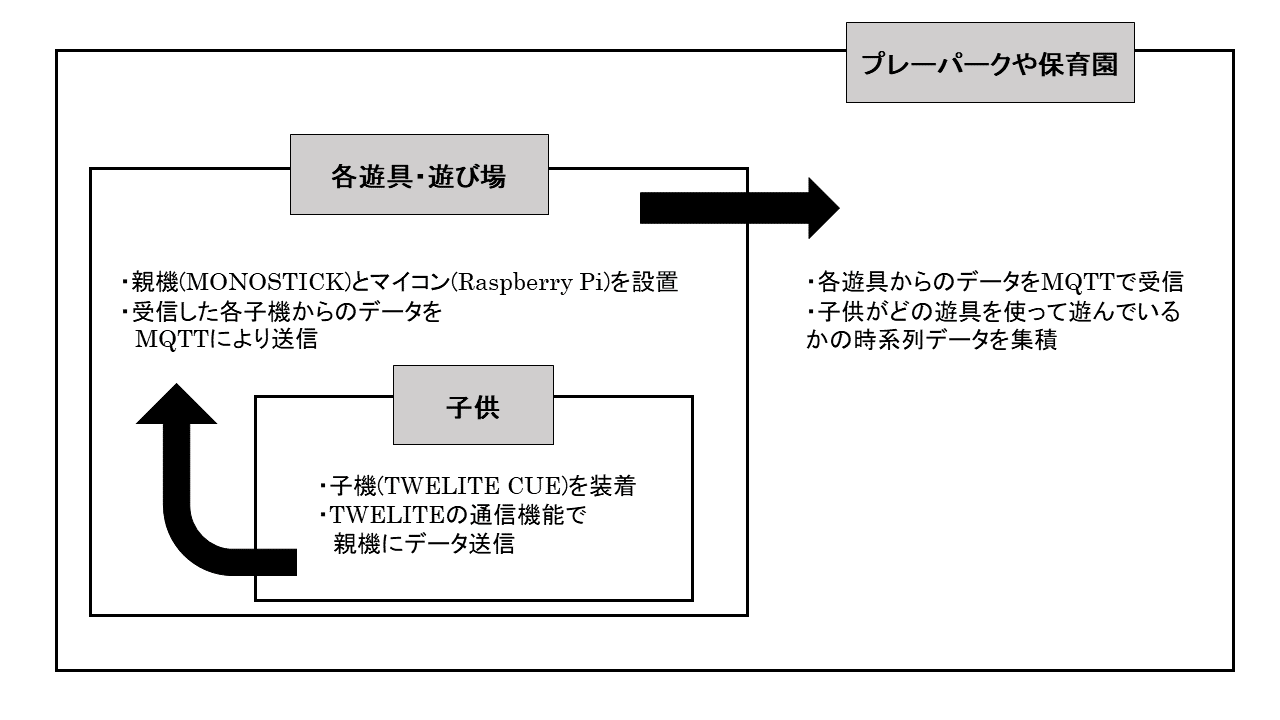
\includegraphics[width = 15.8cm, bb= 0 0 1000 600]{chapter2/kouseigaiyou.png}
  \caption{計測システムの構成}
  \label{system}
\end{figure}







